%%%%%%%%%%%%%%%%%%%%%%%%%%%%%%%%%%%%%%%%%%%%%%%%%%%%%%%%%%%%%%%%%%%%%%%%%%%%%%%%
% Clock
%%%%%%%%%%%%%%%%%%%%%%%%%%%%%%%%%%%%%%%%%%%%%%%%%%%%%%%%%%%%%%%%%%%%%%%%%%%%%%%%
\chapter{Clock} \label{Clock}
\vspace{-10ex}\mCl{syml}\vskip 8ex

%%%%%%%%%%%%%%%%%%%%%%%%%%%%%%%%%%%%%%%%%%%%%%%%%%%%%%%%%%%%%%%%%%%%%%%%%%%%%%%%
% Introduction
%%%%%%%%%%%%%%%%%%%%%%%%%%%%%%%%%%%%%%%%%%%%%%%%%%%%%%%%%%%%%%%%%%%%%%%%%%%%%%%%
\section{Introduction}

This is the mode the device will likely be in a majority of the time.  It
displays the current time and can display the date and current track number
and provides the capability to directly select a track for playback.  It is
also the only mode where you can turn the night light on and off.

\par\medskip

It is the \mPr{f} and \textit{only} mode when the \cRs{f} is in the \dMi{f}
position.

\par\medskip

To get to \mCl{f} mode simply \aTu{f} the \cRs{f} to the \dMi{f}.

\begin{table}[H]
\ers{3}
\centering
\begin{tabu} { X[1,c,m] | X[1,c,m] | X[1,c,m] }
  \thrule
  \thbi{Position} & \thbi{Mode} & \thbi{Action} \\ \mrule
  \sLe & \multirow{2}{*}[-1mm]{\mode{s}{ANY}}
    & $\hskip -4mm$ \sLtoM \\ \dcrule{1}{1} \dcrule{3}{3}
  \sRi & & $\hskip 4mm$ \sRtoM \\ \mdrule
  \sMi & \mCl{sym} & --- \\
  \bhrule
\end{tabu}
\caption{Clock - Mode}
\end{table}

%%%%%%%%%%%%%%%%%%%%%%%%%%%%%%%%%%%%%%%%%%%%%%%%%%%%%%%%%%%%%%%%%%%%%%%%%%%%%%%%
% Overview
%%%%%%%%%%%%%%%%%%%%%%%%%%%%%%%%%%%%%%%%%%%%%%%%%%%%%%%%%%%%%%%%%%%%%%%%%%%%%%%%
\pagebreak
\section{Overview}

There are a number of states the \mCl{f} can be in and are explained in the
following sections.

\begin{table}[H]
\ers{1}
\centering
\begin{tabu} { X[1,c,m] | X[3,l,m] }
  \thrule
  \thbi{State} & \thbi{Description} \\ \mrule
  \sClTi{sym} & Display the current time. \\ \drule{2}
  \sClMD{sym} & Display the month \& day. \\ \drule{2}
  \sClYe{sym} & Display the year.  \\ \drule{2}
  \sClSh{sym} & Display the current track number. \\ \drule{2}
  \sClSe{sym} & Select a track for playback. \\
  \bhrule
\end{tabu}
\caption{Clock - States}
\end{table}

To progress through the states, \aPR{f} the \cEs{f}.  The basic progression from
\sClTi{f} back to \sClTi{f} is:

\as{{ c c c c c c c c c }}{%
\sClTi{sym} & \sPR & \sClMD{sym} & \sPR & \sClYe{sym} & \sPR & \sClSh{sym}
  & \sPR & \sClTi{sym} \\}

\aTo{f} can also be used to show the current track number.  From \sClTi{f},
\sClMD{f} or \sClYe{f}, you will \aTo{f} the \cTo{f} of the enclosure for
\num{1} second to show the current track number.\footnote{ Touch must be enabled
and configured for this to work - see \hyperref[Touch Settings]{\mTS{ss}} for
more information.}

\as{{ c c c }}{%
\sClTi{sym} & & \\ \drule{1}
\sClMD{sym} & \sToN{1} & \sClSh{sym} \\ \drule{1}
\sClYe{sym} & & \\}

At \sClSh{f}, if you \aTu{f} the \cEs{f}, the state will change to \sClSe{f} and
from there you can select a track for playback.

\as{{ c c c }}{\sClSh{sym} & \sTu & \sClSe{sym} \\}

If no action is taken, states other than \sClTi{f} will only display their
values for so many seconds before redisplaying the time.

\as{{ c l l }}{%
\sClMD{sym} & \multirow{2}{*}{\sNPRN{3}}
  & \multirow{8}{*}{\sClTi{sym}} \\ \drule{1}
\sClYe{sym} & & \\ \drule{2}
& \sNPRN{3} & \\ \dcrule{2}{2}
\sClSh{sym}  & \sNTuN{3} & \\ \dcrule{2}{2}
& \sNToN{3} & \\ \drule{2}
& \sNPRN{15} & \\ \dcrule{2}{2}
\sClSe{sym} & \sNTuN{15} & \\ \dcrule{2}{2}
& \sNToN{15} & \\}

%%%%%%%%%%%%%%%%%%%%%%%%%%%%%%%%%%%%%%%%%%%%%%%%%%%%%%%%%%%%%%%%%%%%%%%%%%%%%%%%
% Time
%%%%%%%%%%%%%%%%%%%%%%%%%%%%%%%%%%%%%%%%%%%%%%%%%%%%%%%%%%%%%%%%%%%%%%%%%%%%%%%%
\section{Time} \sClTi{syml}

Displays the current time in either \num{12} or \num{24} hour format, depending
on which was configured via \hyperref[Set Clock]{\mSC{f}}. For \num{12} hour
format, a \textit{decimal} at the \textit{bottom right} of the \cDi{f} is used
to designate \mono{PM}.

\figDT{11:00}{11 AM}{11:00.}{11 PM}

This is the base state of \mCl{f} mode and will be the first when \mCl{f}
mode is selected.  If you go to any other state, you will either need to wait
some amount of time, either \num{3} or \num{15} seconds, or \aPR{f} the \cEs{f}
one or more times. If in \sClSe{f}, after \aPR{f}, the time will redisplay after
\num{3} seconds.  Alternatively, you can \aPR{f} twice to have it redisplay
immediately.

\begin{table}[H]
\ers{0.1}
\centering
\begin{tabu} { c l l }
  \mrule
  \sClMD{sym} & & \multirow{4}{*}{\sClTi{sym}} \\ \drule{1}
  \sClYe{sym} & \sNPRN{3} & \\ \drule{1}
  \sClSh{sym} & & \\ \drule{2}
  \sClSe{sym} & \sNPRN{15} & \\
  \mrule
\end{tabu}
\quad\quad\quad\quad\quad
\begin{tabu} { c l l l }
  \mrule
  \sClMD{sym} & \multicolumn{2}{l}{\sPRN{3}}
    & \multirow{5}{*}{\sClTi{sym}} \\ \drule{3}
  \sClYe{sym} & \multicolumn{2}{l}{\sPRN{2}} & \\ \drule{3}
  \sClSh{sym} & \multicolumn{2}{l}{\sPR} & \\ \drule{3}
  \multirow{2}{*}{\sClSe{sym}} & \sPR & \sNPRN{3} & \\ \dcrule{2}{3}
  & \multicolumn{2}{l}{\sPRN{2}} & \\
  \mrule
\end{tabu}
\end{table}

%%%%%%%%%%%%%%%%%%%%%%%%%%%%%%%%%%%%%%%%%%%%%%%%%%%%%%%%%%%%%%%%%%%%%%%%%%%%%%%%
% Month & Day
%%%%%%%%%%%%%%%%%%%%%%%%%%%%%%%%%%%%%%%%%%%%%%%%%%%%%%%%%%%%%%%%%%%%%%%%%%%%%%%%
\pagebreak
\section{Month \& Day} \sClMD{syml}

Displays the month and day, delimited by a \textit{decimal}.

\figDT{!1.01}{January 1st}{12.31}{December 31st}

To display the month and day from \sClTi{f}, simply \aPR{f} the \cEs{f}.  From
other states, you need to \aPR{f} the \cEs{f} multiple times.

\as{{ c l l }}{%
\sClTi{sym} & \sPR & \multirow{4}{*}{\sClMD{sym}} \\ \drule{2}
\sClSh{sym} & \sPRN{2} & \\ \drule{2}
\sClYe{sym} & \multirow{2}{*}{\sPRN{3}} & \\ \drule{1}
\sClSe{sym} & & \\}

If you don't \aPR{f} the \cEs{f} again within \num{3} seconds, the time will
automatically redisplay.

\as{{ c c c }}{\sClMD{sym} & \sNPRN{3} & \sClTi{sym} \\}

%%%%%%%%%%%%%%%%%%%%%%%%%%%%%%%%%%%%%%%%%%%%%%%%%%%%%%%%%%%%%%%%%%%%%%%%%%%%%%%%
% Year
%%%%%%%%%%%%%%%%%%%%%%%%%%%%%%%%%%%%%%%%%%%%%%%%%%%%%%%%%%%%%%%%%%%%%%%%%%%%%%%%
\section{Year} \sClYe{syml}

Displays the year.

\figDT{2017}{Year 2017}{9999}{Year 9999}

To display the year from \sClMD{f}, simply \aPR{f} the \cEs{f}. From other
states, you need to \aPR{f} the \cEs{f} multiple times.

\as{{c l l }}{%
\sClMD{sym} & \sPR & \multirow{4}{*}{\sClYe{sym}} \\ \drule{2}
\sClTi{sym} & \sPRN{2} & \\ \drule{2}
\sClSh{sym} & \sPRN{3} & \\ \drule{2} 
\sClSe{sym} & \sPRN{4} \\}

If you don't \aPR{f} the \cEs{f} again within \num{3} seconds, the time will
automatically redisplay.

\as{{ c c c }}{\sClYe{sym} & \sNPRN{3} & \sClTi{sym} \\}

%%%%%%%%%%%%%%%%%%%%%%%%%%%%%%%%%%%%%%%%%%%%%%%%%%%%%%%%%%%%%%%%%%%%%%%%%%%%%%%%
% Show Track
%%%%%%%%%%%%%%%%%%%%%%%%%%%%%%%%%%%%%%%%%%%%%%%%%%%%%%%%%%%%%%%%%%%%%%%%%%%%%%%%
\section{Show Track} \label{Show Track} \sClSh{syml}

Displays the current track number that is either playing or poised to play if
paused or stopped.

\figDT{!!!1}{Track \#1}{4096}{Track \#4096}

To display the current track number from \sClYe{f}, simply \aPR{f} the \cEs{f}.
Additionally, after \sClSe{f}, the state goes back to \sClSh{f}.
From other states, you need to \aPR{f} the \cEs{f} multiple times.

\as{{ c l l }}{%
\sClYe{sym} & \multirow{2}{*}{\sPR} & \multirow{4}{*}{\sClSh{sym}} \\ \drule{1}
\sClSe{sym} & & \\ \drule{2}
\sClMD{sym} & \sPRN{2} & \\ \drule{2}
\sClTi{sym} & \sPRN{3} & \\}

\aTo{f} can also be used to display the current track number from \sClTi{f},
\sClMD{f} and \sClYe{f}.  To do so, \aTo{f} the \cTo{f} of the enclosure for
\num{1} second.

\as{{ c c c }}{%
\sClTi{sym} & & \\ \drule{1}
\sClMD{sym} & \sToN{1} & \sClSh{sym} \\ \drule{1}
\sClYe{sym} & & \\}

\info{For \aTo{f} to work, make sure you have enabled it via
\hyperref[Touch Settings]{\mTS{f}} and that the palm of your hand or
most of your fingers lay across the \cTo{f} of the enclosure.}

If you don't \aPR{f} or \aTu{f} the \cEs{f} within \num{3} seconds after
showing the track or aren't touching the \cTo{f} of the enclosure, the time
will automatically redisplay.  If you \aPR{f} before a \aTu{f}, it will
immediately go back to \sClTi{f}.

\as{{ c c c }}{%
\multirow{4}{*}{\sClSh{sym}} & \sPR & \multirow{4}{*}{\sClTi{sym}} \\ \dcrule{2}{2}
& $\hskip 3mm$ \sNTuN{3} & \\ \dcrule{2}{2}
& $\hskip 3mm$ \sNToN{3} & \\ \dcrule{2}{2}
& $\hskip 3mm$ \sNPRN{3} & \\}

It will stay in this state as long as touch is detected\footnote{ If you have
enabled a \textit{Touch Time} via \hyperref[Power Settings]{\mPS{ss}}, the screens
will turn off and the device will sleep if the \textit{Touch Time} is exceeded.}.

%%%%%%%%%%%%%%%%%%%%%%%%%%%%%%%%%%%%%%%%%%%%%%%%%%%%%%%%%%%%%%%%%%%%%%%%%%%%%%%%
% Set Track
%%%%%%%%%%%%%%%%%%%%%%%%%%%%%%%%%%%%%%%%%%%%%%%%%%%%%%%%%%%%%%%%%%%%%%%%%%%%%%%%
\section{Set Track} \label{Set Track} \sClSe{syml}

Allows you to select a track for playback. This can be done
irrespective of \mAu{f} state - it can be in \sAuPl{f}, \sAuPa{f} or
\sAuSt{f}.  This method of selection is also independent of the \mAu{f}
controls - \aPR{f} here will refer to the \cEs{f} and \textit{not} the
\cPl{f} push-button.

\par\medskip

To select a track for playback, you first need to \sClSh{f}. After that, you
need to \aTu{f} the \cEs{f} within \num{3} seconds else it will go back to
\sClTi{f}.

\as{{c c c}}{\sClSh{sym} & \sTuN{3s} & \sClSe{sym} \\}

The idle timeout will be updated to \num{15} seconds after which it will go back
to \sClTi{f}. As long as you are turning the \cEs{f} or touching the \cTo{f} of
the enclosure the timeout will not occur - it is reset with each turn and while
detecting touch.

\as{{l l l}}{%
& \sNTuN{15} & \\ \dcrule{2}{2}
\sClSe{sym} & \sNPRN{15} & \sClTi{sym} \\ \dcrule{2}{2}
& \sNToN{15} & \\}

Continue to \aTu{f} the \cEs{f} until you land on the track number you want
to play - if you turn counter-clockwise past the first track, the number will
wrap to the last track on disk and if you turn clockwise past the last track,
the number will wrap to the first track.  When you're ready, \aPR{f} the
\cEs{f} and the selected track will begin to play and the state will go back to
\sClSh{f}.

\as{{c c c c c}}{%
\multirow{2}{*}{\sClSe{sym}}
  & \sTu & \multirow{2}{*}{\sPR}
  & \multirow{2}{*}{\ePl{sym}{TRACK}} & \multirow{2}{*}{\sClSh{sym}} \\
& \eUp{sym}{} & & & \\}

From \sClSh{f} you can choose to select another track for playback or go back
to displaying the time.  To go back to \sClTi{f}, either

\begin{enumerate}
  \item \aPR{f} the \cEs{f}, \textit{or}
  \item Wait \num{3} seconds.
\end{enumerate}

\info{You must \aTu{f} the \cEs{f} to be able to select a track for playback
even if the current track initially displayed in \sClSh{f} is the track you
want to play since a \aPR{f} of the \cEs{f} will go back to \sClTi{f}.  If the
\mAu{f} is paused or stopped and you want to play the current track that is
poised to play, either
\begin{enumerate}
  \item Press \& Release the \cPl{f} push-button, \textit{or}
  \item \aTu{f} the \cEs{f}, then \aTu{f} back to the current track and \aPR{f}.
\end{enumerate}}

%%%%%%%%%%%%%%%%%%%%%%%%%%%%%%%%%%%%%%%%%%%%%%%%%%%%%%%%%%%%%%%%%%%%%%%%%%%%%%%%
% Night Light
%%%%%%%%%%%%%%%%%%%%%%%%%%%%%%%%%%%%%%%%%%%%%%%%%%%%%%%%%%%%%%%%%%%%%%%%%%%%%%%%
\section{Night Light} \label{Night Light}

One of the main uses of the \cLi{f} window is as a night light. The night
light can only be turned on or off from \mCl{f} mode.  To toggle the night
light on\slash off, \aPH{f} the \cEs{f} for approximately \num{2} seconds.
This is an equivalent hold time for a \aReset{f}, however bars will \textit{not}
blink on the \cDi{f}.

\as{{c c c}}{\state{sym}{ANY STATE} & \sPHN{2} & \eTo{sym}{ON|OFF} \\}

If the \cLi{f} is off, it will turn on\footnote{ The brightness is independent
of this so make sure the \cBr{ss} is turned up.} and if on, it will turn off.

\info{Toggling the night light on/off can be done from \textit{any} state
and will not affect, most importantly, track selection.}

In addition to a white light, up to \num{3} additional colors are configurable
via \hyperref[Set Night Light]{\mSN{f}}.  To select a different night light
color, with the night light on, \aTu{f} the \cEs{f}.

\par\medskip

Because this requires turning the \cEs{f}, it can only be done in \sClTi{f},
\sClMD{f} and \sClYe{f} states.

\as{{c c c c}}{%
\sClTi{sym} & & \\ \dcrule{1}{1}
\sClMD{sym} & \eOn{sym}{NIGHT LIGHT}
  & \sTu & \eAc{sym}{CYCLE COLORS} \\ \dcrule{1}{1}
\sClYe{sym} & & \\}

Note that only unique colors are considered, so if you haven't
configured any of the additional colors there will be no effect.  Also,
duplicate colors are removed from the cycle.

\info{Another way you can achieve turning the night light on and off is to set
one of the configurable colors to black. You can then \aTu{f} the \cEs{f} to
select it, effectively turning the night light off.}

%%%%%%%%%%%%%%%%%%%%%%%%%%%%%%%%%%%%%%%%%%%%%%%%%%%%%%%%%%%%%%%%%%%%%%%%%%%%%%%%
% Night Light - Lighting Animations
%%%%%%%%%%%%%%%%%%%%%%%%%%%%%%%%%%%%%%%%%%%%%%%%%%%%%%%%%%%%%%%%%%%%%%%%%%%%%%%%
\subsection{Lighting Animations}

There are a number of preset, non-configurable lighting animations, in addition
to the solid colors, that you can cycle through.  To toggle between a solid
color light and the lighting animations, \aPH{f} the \cEs{f} for approximately
\num{4} seconds. If the night light is off, it will automatically turn on after
\num{2} seconds as desribed in the previous section.  Continue holding and at
\num{4} seconds it will toggle between a solid color and lighting animation.
However, an unfortunate side effect is that if it is on, it will turn off first
because of the on/off toggle, then turn back on.

\as{{c c c}}{\state{sym}{ANY STATE} & \sPHN{4} & \eTo{sym}{ANIMATION|COLOR} \\}

After toggling the animations on, you can cycle through the different ones in
the same way you can cycle through the solid colors by turning the \cEs{f}.

%%%%%%%%%%%%%%%%%%%%%%%%%%%%%%%%%%%%%%%%%%%%%%%%%%%%%%%%%%%%%%%%%%%%%%%%%%%%%%%%
% Coin Cell Battery
%%%%%%%%%%%%%%%%%%%%%%%%%%%%%%%%%%%%%%%%%%%%%%%%%%%%%%%%%%%%%%%%%%%%%%%%%%%%%%%%
\section{Coin Cell Battery}

There is a \mono{CR2032} \hyperref[Coin Cell Battery]{\cCC{f}}, apart from the
\cRB{f} battery, attached to the \dTo{f} that continues to keep time even when
the device if switched \sOff{f} via the \cPo{f}.  If the time is incorrect when
switching the device \sOn{f}, the battery likely needs replacement.  For more
information see \hyperref[Replacing Battery]{Replacing the Coin Cell Battery}.

%%%%%%%%%%%%%%%%%%%%%%%%%%%%%%%%%%%%%%%%%%%%%%%%%%%%%%%%%%%%%%%%%%%%%%%%%%%%%%%%
% Power
%%%%%%%%%%%%%%%%%%%%%%%%%%%%%%%%%%%%%%%%%%%%%%%%%%%%%%%%%%%%%%%%%%%%%%%%%%%%%%%%
\section{Power}

In \sClTi{f}, \sClMD{f}, \sClYe{f} and \sClSh{f}, the screens will \sDim{f} when
the device enters a \sPoNa{f} power state.

\par\medskip

In \sClTi{f}, \sClMD{f}, \sClYe{f} and \sClSh{f}, the screens will turn \sOff{f}
when the device enters a \sPoSl{f} power state.

\par\medskip

In \sClSe{f}, the device will neither \sPoNa{f} nor \sPoSl{f}.

\ers{2}
\begin{table}[H]
  \begin{tabu}{ X[1,c,m] | X[1,c,m] | X[1,c,m] }
  \thrule
  \thbi{Power State} & \thbi{Clock State} & \thbi{Screens} \\ \mrule

  \multirow{2}{*}[-1mm]{\sPoNa{sym}} 
    & \sClTi{sym} \sClMD{sym} \sClYe{sym} \newline \sClSh{sym}
    & \sDim{sym} \\ \dcrule{2}{3}
  & \sClSe{sym} & \sOn{sym} \\ \mrule

  \multirow{2}{*}[-1mm]{\sPoSl{sym}} 
    & \sClTi{sym} \sClMD{sym} \sClYe{sym} \newline \sClSh{sym}
    & \sOff{sym} \\ \dcrule{2}{3}
  & \sClSe{sym} & \sOn{sym} \\

  \bhrule
  \end{tabu}
\caption {Clock - Power}
\end{table}

%%%%%%%%%%%%%%%%%%%%%%%%%%%%%%%%%%%%%%%%%%%%%%%%%%%%%%%%%%%%%%%%%%%%%%%%%%%%%%%%
% Reference
%%%%%%%%%%%%%%%%%%%%%%%%%%%%%%%%%%%%%%%%%%%%%%%%%%%%%%%%%%%%%%%%%%%%%%%%%%%%%%%%
\pagebreak
\section{Reference} \label{Clock - Reference}

\ers{3}
\begin{longtabu}{ X[2,c,m] | X[1,c,m] | X[4,c,m] | X[2,c,m] }
  \thrule
  \thbi{State} & \thbi{Action} & \thbi{Effect} & \thbi{Next} \\ \mdrule

  \multirow{3}{*}[-1.5mm]{\sClTi{sym}}
    & \sPR & \eDi{sym}{MONTH \& DAY} & \sClMD{sym} \\ \dcrule{2}{4}
  & \sToN{1} & \eDi{sym}{TRACK} & \sClSh{sym} \\ \dcrule{2}{4}
  & \sTu & \eAc{sym}{CYCLE NL} & --- \\ \mrule

  \multirow{4}{*}[-1.5mm]{\sClMD{sym}}
    & \sPR & \eDi{sym}{YEAR} & \sClYe{sym} \\ \dcrule{2}{4}
  & \sToN{1} & \eDi{sym}{TRACK} & \sClSh{sym} \\ \dcrule{2}{4}
  & \sNPRN{3} & \eDi{sym}{TIME} & \sClTi{sym} \\ \dcrule{2}{4}
  & \sTu & \eAc{sym}{CYCLE NL} & --- \\ \mrule

  \multirow{4}{*}[-1.5mm]{\sClYe{sym}}
    & \sPR & \multirow{2}{*}[-1mm]{\eDi{sym}{TRACK}}
    & \multirow{2}{*}[-1mm]{\sClSh{sym}} \\ \dcrule{2}{2}
  & \sToN{1} & & \\ \dcrule{2}{4}
  & \sNPRN{3} & \eDi{sym}{TIME} & \sClTi{sym} \\ \dcrule{2}{4}
  & \sTu & \eAc{sym}{CYCLE NL} & --- \\ \mrule

  \pagebreak
  \mrule

  & \sTu & \eUp{sym}{TRACK} & \sClSe{sym} \\ \dcrule{2}{4}
  & \sPR & \multirow{4}{*}[-1.5mm]{\eDi{sym}{TIME}}
    & \multirow{4}{*}[-1.5mm]{\sClTi{sym}} \\ \dcrule{2}{2}
  \sClSh{sym} & \sNTuN{3} & & \\ \dcrule{2}{2}
  & \sNPRN{3} & & \\ \dcrule{2}{2}
  & \sNToN{3} & & \\ \mrule

  & \sTu & \eUp{sym}{TRACK} & --- \\ \dcrule{2}{4}
  & \sPR & \ePl{sym}{TRACK} & \sClSh{sym} \\ \dcrule{2}{4}
  \sClSe{sym} & \sNTuN{15} & & \\ \dcrule{2}{2}
  & \sNPRN{15} & \eDi{sym}{TIME} & \sClTi{sym} \\ \dcrule{2}{2}
  & \sNToN{15} & & \\ \mrule

  \multirow{4}{*}{\state{f}{ANY}}
    & $\hskip 2.5mm$ \sPHN{2} & \eTo{sym}{NL ON|OFF} & --- \\ \dcrule{2}{4}
  & $\hskip 2.5mm$ \sPHN{4}
    & \eTo{sym}{NL COLOR|ANIMATION} & --- \\ \dcrule{2}{4}
  & $\hskip -3.5mm$ \sMtoL & \multirow{2}{*}[-1mm]{\eCM{sym}}
    & \mSA{sym} \\ \dcrule{2}{2} \dcrule{4}{4}
  & $\hskip 3.5mm$ \sMtoR & & \mTi{sym} \\

  \bhrule
  \caption {Clock - Reference}
\end{longtabu}

%%%%%%%%%%%%%%%%%%%%%%%%%%%%%%%%%%%%%%%%%%%%%%%%%%%%%%%%%%%%%%%%%%%%%%%%%%%%%%%%
% State Diagram
%%%%%%%%%%%%%%%%%%%%%%%%%%%%%%%%%%%%%%%%%%%%%%%%%%%%%%%%%%%%%%%%%%%%%%%%%%%%%%%%
%\pagebreak
\section{State Diagram} \label{Clock State Diagram}

\begin{figure}[H]
  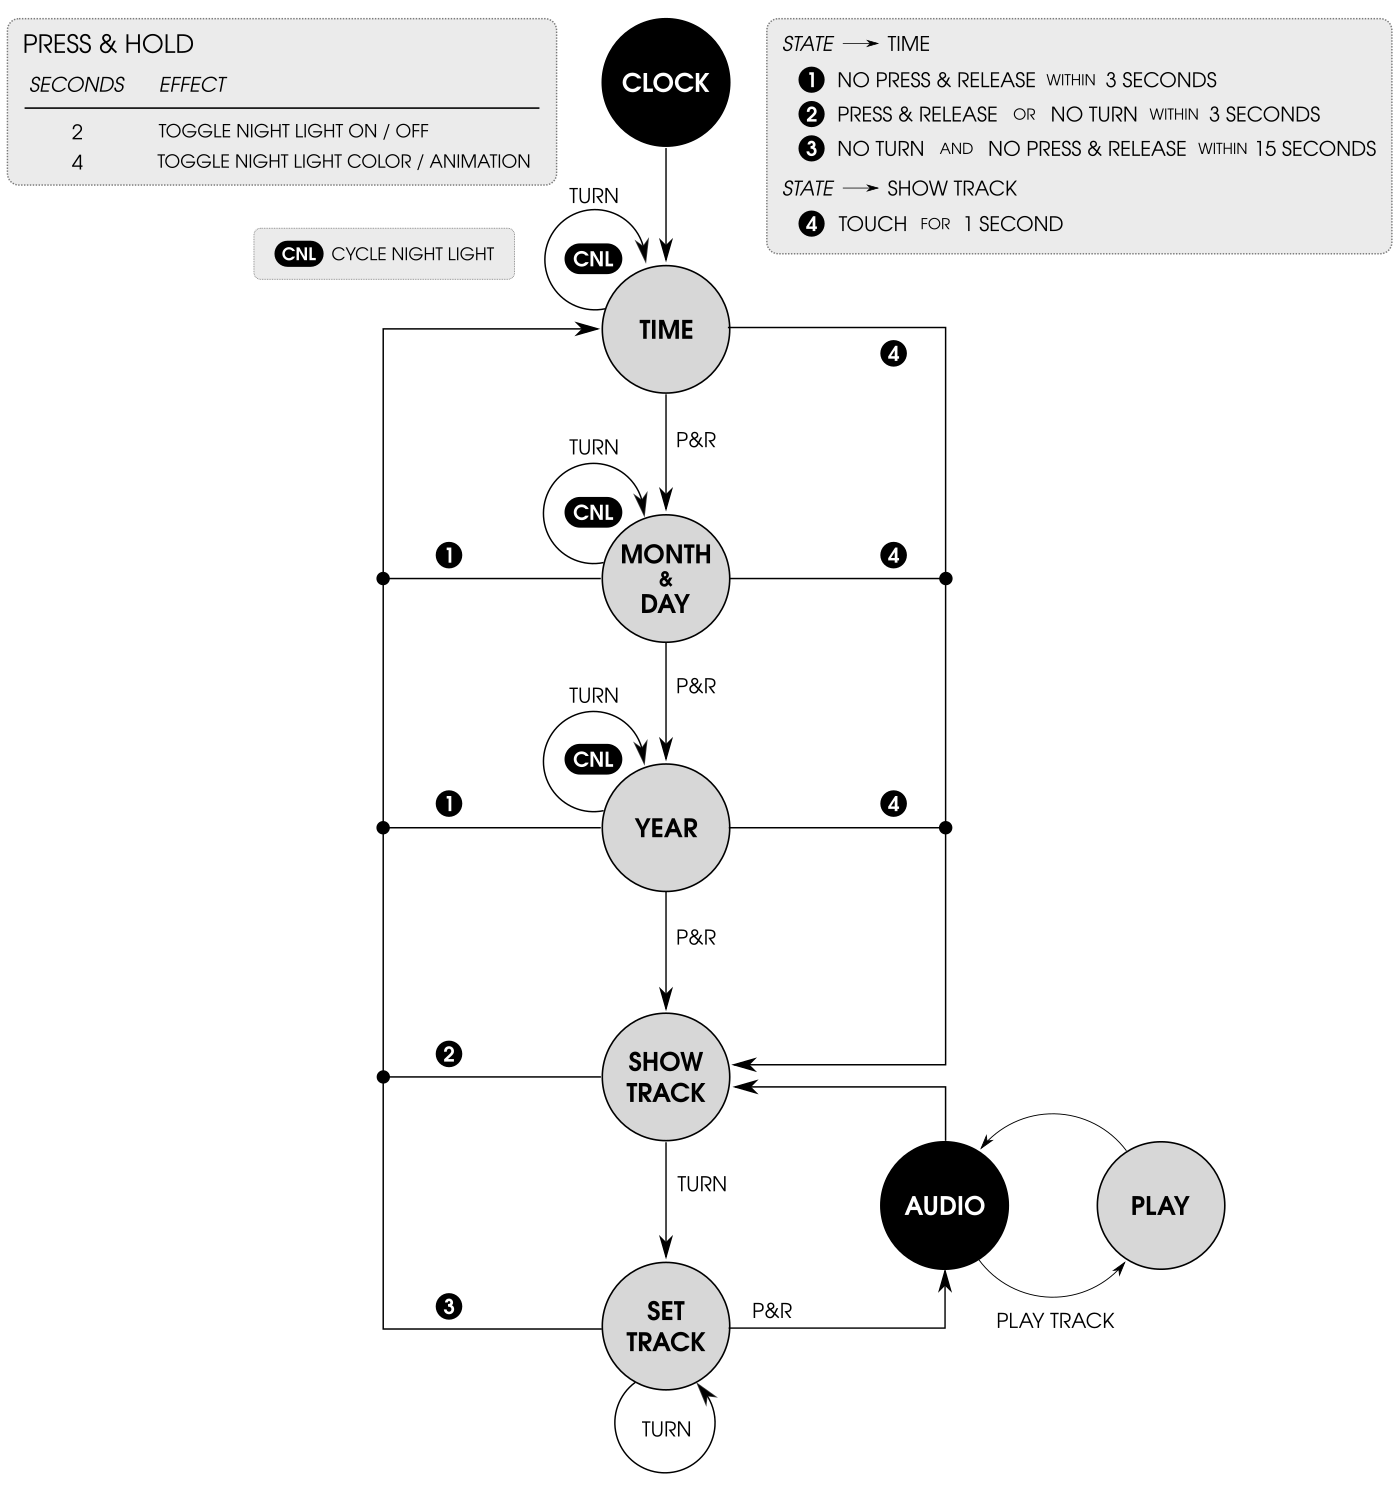
\includegraphics[]{images/clock_state_diagram.png}
\caption{Clock - State Diagram}
\end{figure}
